\subsection{Formula del punto medio composita}

Data la proprietà di additività dell'integrale:
\begin{equation*}
	I\left(f\right) = \displaystyle\sum_{k=1}^{M} \int_{I_{k}} f\left(x\right) \:\mathrm{d}x
\end{equation*}
Si possono approssimare il valore dell'integrale su ogni intervallo e dopodiché sommare i contributi.

\highspace
Per cui, l'idea del \definition{punto medio composita} è quella di approssimare il valore dell'integrale della funzione:
\begin{equation*}
	\int_{I_{k}} f\left(x\right) \:\mathrm{d}x
\end{equation*}
Con l'area del rettangolo con altezza $f\left(\overline{x}_{k}\right)$:
\begin{figure}[!htp]
	\centering
	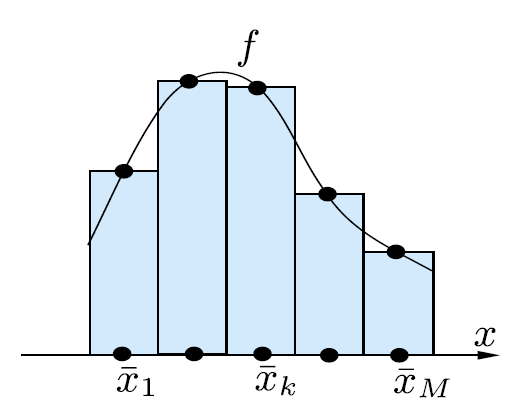
\includegraphics[width=.4\textwidth]{img/formule-di-quadratura-2.png}
\end{figure}

\noindent
Dato che l'altezza dei rettangoli è sempre pari ad $H$, si avrà la seguente approssimazione per $I\left(f\right)$:
\begin{equation}
	I_{pm}\left(f\right) = H \displaystyle\sum_{k=1}^{M} f\left(\overline{x}_{k}\right)
\end{equation}
Dove $pm$ indica \emph{punto medio}.

\highspace
Inoltre, la \definition{stima dell'errore del punto medio composita} è:
\begin{equation}
	\left|I\left(f\right) - I_{pm}\left(f\right)\right| \le \underset{x}{\max}\left|f'' \left(x\right)\right| \: \dfrac{b-a}{24} H^{2}
\end{equation}
Si possono fare due \textbf{osservazioni} interessanti su questa stima dell'errore:\\
\begin{enumerate}
	\item La formula del \textbf{punto medio composita} è di \textbf{ordine 2}.
	
	\item La formula del \textbf{punto medio composita} ha \textbf{grado di esattezza pari a 1}. Dato che è stata assunta la continuità della derivata seconda di $f$, allora $f''=0$ in ogni $x$ se $f$ è una retta, ovverosia con $r=1$.
\end{enumerate}
Dall'ultima osservazione, risulta chiaro che la \textbf{formula del punto medio composita è esatta se applicata alle rette}.